\section{}
Recall the rolling-cylinder-on-a-board system from Assignment \#1:
\begin{figure}[h]
    \centering
    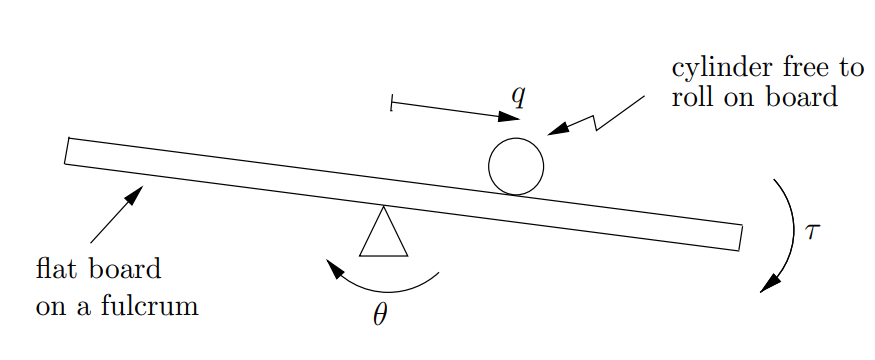
\includegraphics[width=0.5\textwidth]{Questions/Figures/Q2ProblemDiagram.png}
    \caption{Rolling cylinder on a board.}
    \label{fig:Q2 System}
\end{figure}

% In Assignment#1, defining the state vector x = (x1, x2, x3, x4) = (q, θ, q,˙
% ˙θ), input u = τ and output
% y = q, you obtained the state model

In Assignment \#1, defining the state vector $x = [x_1, x_2, x_3, x_4] = 
[q, \theta, \dot{q}, \dot{\theta}]$, input $u = \tau$ and output $y = q$, you obtained the state model
\[
    \begin{aligned}
        \dot{x} &=
        \begin{bmatrix}
            x_3 \\
            x_4 \\
            \frac{-M_c g \sin x_2 + M_c x_1 x_4^2}{\frac{J_c}{R_c^2} + M_c} \\
            \frac{- 2M_c x_1 x_3 x_4 - M_c g x_1 \cos x_2 + u}{M_c x_1^2 + J + J_c}
        \end{bmatrix} 
            = f(x, u) \\
        y &= x_1
    \end{aligned}
\]

\subsection{}
\textit{Find the two equilibrium points of this system}

An equilibrium point is defined as a state $x_0 = [x_{10}, x_{20}, x_{30}, x_{40}]$ and input $u_0$ that satisfies $f(x_0, u_0) = 0$. 
Working through some algebra, we get the following the following observations:
\[
    \begin{aligned}
        &x_{30} = 0 \\
        &x_{40} = 0 \\
        &\frac{-M_c g \sin x_{20} + \cancel{M_c x_{10} x_{40}^2}}{\frac{J_c}{R_c^2} + M_c} = 0 \\
        &\frac{\cancel{- 2M_c x_{10} x_{30} x_{40}} - M_c g x_{10} \cos x_{20} + u_0}{M_c x_{10}^2 + J + J_c} = 0 \\
        &\dot{x_{10}} = 0
    \end{aligned}
\]

We see that $x_{30} = x_{40} = 0$ and $x_{10} \in \mathbb{R}$. Next, solve for $x_{20}$:
\[
    \begin{aligned}
        \frac{-M_c g \sin x_{20}}{\frac{J_c}{R_c^2} + M_c} &= 0 \\
        \implies \sin x_{20} &= 0 \\
        x_{20} &= 0, \pi
    \end{aligned}
\]

Finally, solve for $u_0$:
\[
    \begin{aligned}
        \frac{- M_c g x_{10} \cos x_{20} + u_0}{M_c x_{10}^2 + J + J_c} &= 0 \\
        \implies u_0 &= M_c g x_{10} \cos x_{20} \\
        u_0 &= \pm M_c g x_{10}
    \end{aligned}
\]

Therefore, the two equilibrium points are:
\begin{empheq}[box=\fbox]{align*}
        x_{0,1} &= [x_{10}, 0, 0, 0] \\
        u_{0,1} &= M_c g x_{10} \\
        x_{0,2} &= [x_{10}, \pi, 0, 0] \\
        u_{0,2} &= -M_c g x_{10}
\end{empheq}

\subsection{}
\textit{One of these is mathematically valid but not physically relevant. Which one and why?}'

The second equilibrium point is not physically relevant because the fulcrum limits the range of motion of the board. In addition, by the time the 
board reaches $\theta = \pi$, the cylinder would have rolled off the board.

\subsection{}
\textit{Using MATLAB, linearize the system about the relevant equilibrium point and give the corresponding A, B, C and D matrices.}

By Matlab,

\begin{empheq}[box=\fbox]{align*}
    A &=
    \begin{bmatrix}
        0 & 0 & 1 & 0 \\
        0 & 0 & 0 & 1 \\
        0 & -\frac{M_c g}{M_c + \frac{J_c}{R_c^2}} & 0 & 0 \\
        -\frac{M_c g}{M_c x_{10}^2 + J + J_c} & 0 & 0 & 0
    \end{bmatrix} \\
    B &=
    \begin{bmatrix}
        0 \\
        0 \\
        0 \\
        \frac{1}{M_c x_{10}^2 + J + J_c}
    \end{bmatrix} \\
    C &=
    \begin{bmatrix}
        1 & 0 & 0 & 0
    \end{bmatrix} \\
    D &= 0
\end{empheq}

The Matlab code used to generate the above matrices is shown below:
\lstinputlisting[language=Matlab]{Questions/Code/a2q2.m}